%%%%%%%%%%%%%%%%%%%%%%%%%%%%%%%%%%%%%%%%%%%%%%%%%%%
%% P3: Phenomenology of Particle Physics                         
%%
%% Author:  André Rubbia                   		 
%%
%% Figure 16.11 Measured total cross-section $\sigma$ normalized to the Mott cross-section vs. $Q^2$.
%%
%% This work is licensed under the Creative Commons Attribution 4.0 International License. 
%% To view a copy of this license, visit http://creativecommons.org/licenses/by/4.0/ or 
%% send a letter to Creative Commons, PO Box 1866, Mountain View, CA 94042, USA.
%%
%%%%%%%%%%%%%%%%%%%%%%%%%%%%%%%%%%%%%%%%%%%%%%%%%%%

\documentclass[a4paper,10pt]{article}

\usepackage[T1]{fontenc}
\usepackage[utf8]{inputenc}
\usepackage{lmodern}
\usepackage[labelfont=bf]{caption}
\usepackage{upgreek}

\usepackage{tikz}
\usepackage{pgfplots}
\pgfplotsset{compat=1.17}
\usepgfplotslibrary{ternary}
\usepgfplotslibrary{fillbetween}
\usepgfplotslibrary{external}

\def\d{\mathrm{d}}

\begin{document}

%%%%%%%%%%%%%%%   FIGURE  %%%%%%%%%%%%%%%%%%%%%%%%%%%%%%
\begin{figure}[htb]
\begin{center}
%%%%\includegraphics[width=0.3\textwidth]{Figures/ElectronProtonScatt/inelasticep_sigmavsmott.pdf}
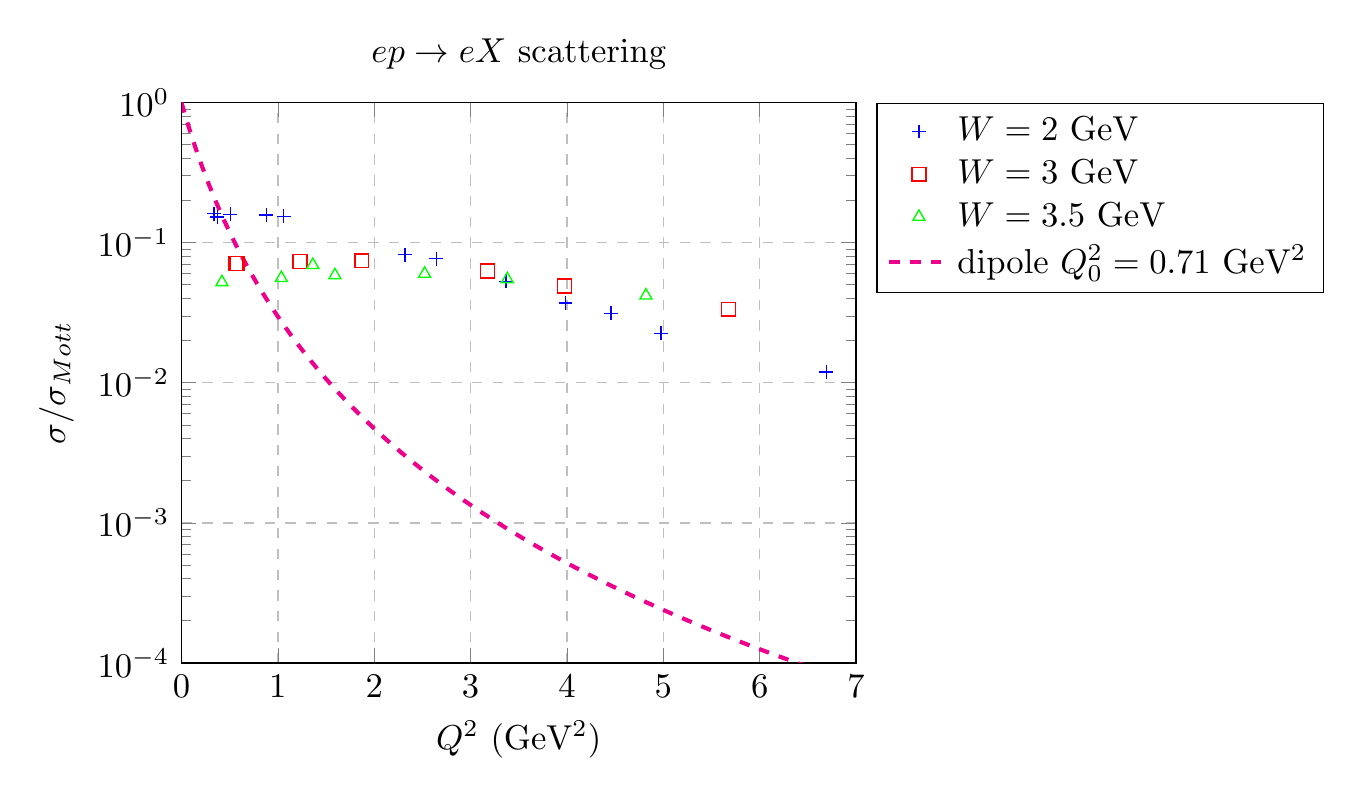
\begin{tikzpicture}[scale=1.25]
\begin{semilogyaxis}[
    title={$ep\rightarrow eX$ scattering},
    xlabel={$Q^2$  (GeV$^2$)},
    ylabel={$\sigma/\sigma_{Mott}$},
    xmin=0, xmax=7,
    ymin=1e-4, ymax=1,
%    xtick={0,20,40,60,80,100,120,140,160},
%    tick={1e0,1e1,1e2,1e3,1e4,1e5,1e6,1e7},
	legend style={legend pos = outer north east},
	legend cell align = {left},
    	ymajorgrids=true,
    	xmajorgrids=true,
    grid style=dashed,
]

%%    W=2GeV
\addplot[
    color=blue,
    mark=+,
    only marks,
    error bars/.cd,
    y dir=both, y explicit
    ]
    coordinates {
(0.33612,0.161098)
(0.37231,0.152277)
(0.50536,0.159335)
(0.88013,0.157644)
(1.06145,0.154175)
(2.31796,0.082171)
(2.6443,0.076837)
(3.3692,0.053029)
(3.98531,0.037006)
(4.45659,0.031272)
(4.97603,0.022571)
(6.69194,0.0119034)
};

%%    W=3GeV
\addplot[
    color=red,
    mark=square,
    only marks,
    error bars/.cd,
    y dir=both, y explicit
    ]
    coordinates {
(0.56474,0.070769)
(0.57683,0.070771)
(1.22973,0.073282)
(1.87051,0.074189)
(3.17599,0.062779)
(3.97359,0.049053)
(5.67775,0.033527)
};

%%    W=3.5GeV
\addplot[
    color=green,
    mark=triangle,
    only marks,
    error bars/.cd,
    y dir=both, y explicit
    ]
    coordinates {
(0.41927,0.052186)
(1.03594,0.055893)
(1.36264,0.06928)
(1.59213,0.058524)
(2.52308,0.059948)
(3.38134,0.054854)
(4.81967,0.041948)
};


%% elastic
\addplot[domain=0:7,
    color=magenta,
    no marks, very thick, dashed,
    samples=100
    ] {1.0/(1.0+(x/0.71))^4};


      \legend{$W=2$~GeV, $W=3$~GeV, $W=3.5$~GeV, dipole $Q_0^2=0.71$~GeV$^2$}
\end{semilogyaxis}
\end{tikzpicture}
\caption{Measured total cross-section $\sigma$ normalized
to the Mott cross-section vs. $Q^2$.  There is a striking difference between
the data at the chosen $W$ values and the elastic cross-section illustrated
by the dipole form. No errors on the data are displayed.
Data reprinted with permission from
M.~Breidenbach {\em et~al.}, ``Observed behavior of highly inelastic
  electron--proton scattering,'' {\em Phys. Rev. Lett.}, vol.~23, pp.~935--939,
  Oct 1969.}
\end{center}
\end{figure}
%%%%%%%%%%%%%%%  END FIGURE  %%%%%%%%%%%%%%%%%%%%%%%%%%%%%%
%

\end{document}
